% Präambel
\documentclass[12pt,a4paper,oneside, 
liststotoc, 					% Tabellen- und Abbildungsverzeichnis ins Inhaltsverzeichnis
bibtotoc,						% Literaturverzeichnis ins Inhaltsverzeichnis aufnehmen
titlepage, 						% Titlepage-Umgebung statt \maketitle
headsepline, 					% horizontale Linie unter Kolumnentitel
%abstracton,					% Überschrift beim Abstract einschalten, Abstract muss dazu in {abstract}-Umgebung stehen
%DIV11,							% auskommentieren, um den Seitenspiegel zu vergrößern
BCOR6mm,						% Bindekorrektur, die den Seitenspiegel um 6mm nach rechts verschiebt,
openany,							% Unterdrückung von leeren Seiten nach Chapter-Ende
]{scrreprt}			
%\usepackage{utf8} 				% Dokument in utf8-Codierung schreiben und speichern
\usepackage[utf8]{inputenc} 	% ermöglicht die direkte Eingabe von Umlauten
\usepackage[paper=a4paper,left=30mm,right=25mm,top=30mm,bottom=30mm]{geometry} % seitenabstand
\usepackage[ngerman]{babel} 	% deutsche Trennungsregeln und Übersetzung der festcodierten Überschriften
\usepackage[T1]{fontenc} 		% Ausgabe aller zeichen in einer T1-Codierung (wichtig für die Ausgabe von Umlauten!)
\usepackage{graphicx}  			% Einbinden von Grafiken erlauben
%\usepackage{amsmath}
%\usepackage{amsfonts}
%\usepackage{amssymb}
\usepackage{mathpazo} 			% Einstellung der verwendeten Schriftarten
\usepackage{textcomp} 			% zum Einsatz von Eurozeichen u. a. Symbolen
\usepackage{listings}			% Datstellung von Quellcode mit den Umgebungen {lstlisting}, \lstinline und \lstinputlisting
\usepackage{xcolor} 			% einfache Verwendung von Farben in nahezu allen Farbmodellen
\usepackage[intoc]{nomencl} 	% zur Erstellung des Abkürzungsberzeichnisses
\usepackage{fancyhdr}			% Zusatzpaket zur Gestaltung von Fuß und Kopfzeilen
% persönliche Packages:
\usepackage{subfigure} 			% 2 Bilder nebeneinander
\usepackage{placeins}
\usepackage[onehalfspacing]{setspace} % Zeilenabstand
% Litaraturverzeichnis:
\usepackage[backend=bibtex,style=authoryear-icomp]{biblatex}
\usepackage[babel,german=guillemets]{csquotes}
\usepackage{acronym} % Abkürzungsverzeichnis
\bibliography{Inhalt/literatur.bib}
\nocite{*}
% Java Code:
\usepackage{color}

\definecolor{dkgreen}{rgb}{0,0.6,0}
\definecolor{gray}{rgb}{0.5,0.5,0.5}
\definecolor{mauve}{rgb}{0.58,0,0.82}

\lstset{frame=tb,
  language=Java,
  aboveskip=3mm,
  belowskip=3mm,
  showstringspaces=false,
  columns=flexible,
  basicstyle={\small\ttfamily},
  numbers=none,
  numberstyle=\tiny\color{gray},
  keywordstyle=\color{blue},
  commentstyle=\color{dkgreen},
  stringstyle=\color{mauve},
  breaklines=true,
  breakatwhitespace=true,
  tabsize=3
}
% -----------------------------------------------------------------------------------------------------------------
% Zum Aktualisieren des Abkürzungsverzeichnisses bitte auf der Kommandozeile folgenden Befehl aufrufen :
%  makeindex Bachelorarbeit.nlo -s nomencl.ist -o Bachelorarbeit.nls 
%  

% Schneller Compiler (bibtex, akürzungen, latex, pdf anzeigen im internen fenster (texmaker))
% 	makeindex Bachelorarbeit.nlo -s nomencl.ist -o Bachelorarbeit.nls | bibtex %|pdflatex -synctex=1 -interaction=nonstopmode %.tex|"C:/Program Files (x86)/Adobe/Reader 11.0/Reader/AcroRd32.exe" %.pdf
% 
% einfach in Bachelorarbeit.tex ausführen -----------------------------------------------------------------------------------------------------------------

%usepackage float mit H für Bilder

% Hier die persönlichen Daten eingeben:

\newcommand{\titel}{Frontend Webentwicklung}
\newcommand{\untertitel}{eines Internet of Things Showcases am Beispiel von Connected Cars}
\newcommand{\arbeit}{Praxisbericht}
\newcommand{\prufungvortext}{T2000}
\newcommand{\prufung}{Bericht über PE 3/4} 
\newcommand{\studiengang}{Angewandte Informatik}
\newcommand{\autor}{Robin Schlenker}
\newcommand{\matrikelnr}{2006895}
\newcommand{\kurs}{TINF14A}
\newcommand{\firma}{IBM Deutschland GmbH}
\newcommand{\abgabe}{\today}
\newcommand{\betreuerdhbw}{unbekannt}

\newcommand{\jahr}{2015}			% für Angabe im Copyright-Vermerk der Titelseite

% Abkürzungen
\newcommand{\ua}{\mbox{u.\,a.\ }}
\newcommand{\zb}{\mbox{z.\,B.\ }}
\newcommand{\bs}{$\backslash$}

\renewcommand{\nomname}{Abkürzungsverzeichnis}

% -------------------------------------------------------------------------------------------
% Definition der Kopf- und Fußzeilen
\lhead{}								% Kopf links
\chead{}								% Kopf mitte
\rhead{\sffamily{Frontendentwicklung IoT ConnectedCars}}				% Kopf rechts
\lfoot{\prufungvortext}					% Fuß links
\cfoot{\sffamily{\thepage}}				% Fuß mitte
\rfoot{\sffamily{\autor}}				% Fuß rechts
\renewcommand{\headrulewidth}{0.4pt}	% Liniendicke Kopf
\renewcommand{\footrulewidth}{0.4pt}	% Liniendicke Fuß


\makenomenclature							% Abkürzungsverzeichnis erstellen

% alle Abkürzungen, die in der Bachelorarbeit verwendet werden

\nomenclature{DHBW}{Duale Hochschule Baden-Württemberg}
\nomenclature{IoT}{Internet of Things}
\nomenclature{MVC}{Model-View-Controller}
% -------------------------------------------------------------------------------------------
%                     Beginn des Dokumenteninhalts
% -------------------------------------------------------------------------------------------
\begin{document}
\setcounter{secnumdepth}{4}					% Nummerierungstiefe fürs Inhaltsverzeichnis
\setcounter{tocdepth}{2}
\sffamily									% für die Titelei serifenlose Schrift verwenden

% ------------------------------ Titelei -----------------------------------------------------

\thispagestyle{plain}
\begin{titlepage}
\enlargethispage{4.0cm}
\sffamily 								% Serifenlose Grundschrift für die Titelseite einstellen

\singlespacing
\begin{figure}
	\hspace{-2.0cm}
    \hspace{7cm}
    \subfigure{
\includegraphics[scale=2.0]{Bilder/logo_dhbw.jpg}\\[5ex]}
\end{figure} 


\begin{center}

\huge{\textsc{\textbf{\titel}}}\\[1.5ex]
\Large{\textbf{\untertitel}}\\[5ex]
\LARGE{\textbf{\arbeit}}\\[2ex]
\Large{Studiengang \studiengang}\\[1ex]
\normalsize{Duale Hochschule Baden-Württemberg Stuttgart}\\[5ex]

\end{center}

\begin{flushleft}
\begin{tabular}{ll}
Abgabedatum:					& \quad \abgabe \\
Matrikelnummer, Kurs: 			& \quad \matrikelnr , \kurs \\ 
Gutachter der Dualen Hochschule: & \quad \betreuerdhbw \\ [5ex]

\end{tabular} 

\end{flushleft}

\end{titlepage} 				% erzeugt die Titelseite
\pagenumbering{Roman}						% große, römische Seitenzahlen für Titelei	
\addchap*{Eidesstattliche Erklärung}
Ich versichere hiermit, dass ich meine Arbeit mit dem Thema
\begin{quote}
\textit{\titel} -\textit{ \untertitel }
\end{quote}
selbständig verfasst und keine anderen als die angegebenen Quellen und Hilfsmittel benutzt habe. Die Arbeit wurde bisher keiner anderen Prüfungsbehörde vorgelegt und auch nicht veröffentlicht.  \\[10ex]


% Mir ist bekannt, dass ich meine Diplomarbeit zusammen mit dieser Erklärung fristgemäß nach Vergabe des Themas in dreifacher Ausfertigung und gebunden im Sekretariat meines Studiengangs an der DHBW Karlsruhe abzugeben habe. Als Abgabetermin giltbei postalischer Übersendung der Eingangsstempel der DHBW, also nicht der Poststempel oder der Zeitpunkt eines Einwurfs in einen Briefkasten der DHBW.


Stuttgart, den \today \\[4ex]

%\includegraphics[scale=1]{unterschrift.png}\\[-5ex]
\rule[0.2cm]{8cm}{0.5pt} \\
\textsc{\autor} ~ \textit{ (\matrikelnr)} \\[10ex]

% Sperrvermerk bei Bedarf dekommentieren
\hrule 
\vspace*{1.0cm}
\noindent \textbf{\Large{Sperrvermerk}}\\
\normalsize
\textbf{Die Ergebnisse der Arbeit stehen ausschließlich dem auf dem Deckblatt aufgeführten Ausbildungsbetrieb, der \firma , zur Verfügung.} 				% Einbinden der eidestattlichen Erklärung
\addchap{Abstract} %*-Variante sorgt dafür, das Abstract nicht im Inhaltsverzeichnis auftaucht

Abstract Lorem ipsum   				% Einbinden des Abstracts

\singlespacing
\tableofcontents							% Erzeugen des Inhalsverzeichnisses
\onehalfspacing
\printnomenclature[2.0cm]					% Erzeugen des Abkürzungsverzeichnisses
\listoffigures 								% Erzeugen des Abbildungsverzeichnisses 

\listoftables 								% Erzeugen des Tabellenverzeichnisses
\pagebreak

% --------------------------------------------------------------------------------------------
%                    Inhalt der Bachelorarbeit
%---------------------------------------------------------------------------------------------
\pagenumbering{arabic}						% arabische Seitenzahlen für den Hauptteil
\pagestyle{fancy}					
\rmfamily

\chapter{Einleitung}
Die Web-Entwicklung ist wohl eine der sich am schnellsten verändernden IT Herausforderungen. Nur wenige Bereiche der Programmierung haben sich in den letzten 10 Jahren so rasant verändert wie die Entwicklung von Internet-Auftritten und der damit zusammenhängenden Infrastruktur. So waren die meisten Web-Auftritte im Web 1.0 ( bis ca. 2000) noch vorwiegend von statischen Webseiten geprägt. 
„Da als Ziel zunächst nur galt, statische Dokumente abbilden zu können, waren die ersten Webseiten ebenso: statisch. Dies spiegelt sich bis heute in der Natur von HTML wider, das ohne Zuhilfenahme weiterer Technologien lediglich zur Darstellung rein statischer Inhalte taugt.“\footcite{nodejsroden}
Als dann unter anderem mit Javascript die Möglichkeit der Dynamisierung in die Webentwicklung eintrat, wurden die Anforderungen an Webseiten sehr schnell viel höher als nur wenige Jahre zuvor. Dies war nicht nur für die Bewältigung nie gekannter Daten-Mengen im Backend eine enorme Herausforderung, sondern auch die Entwicklung von Benutzeroberflächen und deren Infrastruktur gestaltete sich immer komplexer und facettenreicher. Gerade Webseiten, die nicht ausschließlich der Darstellung von statischen Inhalten dienen benötigten neue Grund-Strukturen zur Datenübermittlung und Verarbeitung. Diese Anforderungen zu erfüllen ist nun eine Herausforderung der sich immer mehr Entwickler stellen müssen. Dadurch entstanden beziehungsweise entstehen immer noch eine Unmenge von Möglichkeiten das Frontend einer Webseite zu entwickeln. Da die Anforderungen an Webseiten auch in jedem Einzelfall zu unterscheiden sind ist eine wichtige Aufgabe der Webseiten-Entwicklung die Evaluierung des Kontextes, der Anforderungen und der passenden Frameworks. Diese Projekt-Arbeit verfolgt ebenjenes Ziel der Markt-Analyse und Umsetzung eines Projekts dass sich im Bereich Internet of Things ansiedelt. Die Arbeit befasst sich mit den Anforderungen die sich speziell für IoT Web-Anwendungen ergeben und evaluiert dann am Beispiel einer Connected Cars Anwendung die benötigten Frameworks. Auf die Umsetzung des Backends wird die Arbeit nicht eingehen. 

%--------- Kontext und Anforderungen ---------%

\chapter{ Kontext und Anforderungen}\label{context}
Dieses Kapitel beschäftigt sich mit dem Kontext der Beispiel-Anwendung, im Folgenden CarConnect, und die für IoT-Showcases benötigten Anforderungen im Allgemeinen.
\subsubsection{Wirtschaftlicher Kontext}\label{context_business}
Bei der Beispiel-Anwendung handelt es sich um eine Web-Applikation die es sich zur Aufgabe macht, Sensordaten von Kraftfahrzeugen auszuwerten und entsprechend dazustellen. Ziel ist es einerseits, die Möglichkeiten der IBM IoT-Abteilung sichtbar zu machen sowie andererseits auch für die Wirtschaft die Möglichkeiten von verknüpften Fahrzeugen dazulegen.\\
Ein Automobil-Hersteller sollte erkennen, dass die Sammlung von Sensoren-Daten für ihn immense Vorteile erwirtschaften könnte. So wäre er mit den erhobenen Daten unter anderem in der Lage herauszufinden, in welcher Region seine Autos fahren beziehungsweise welches seiner Modelle wo bevorzugt wird. Dies würde ihm ermöglichen, seine Infrastruktur zu optimieren. Aber auch das Stichwort "Predictive Maintenance", also vorhersehende Instandhaltung spielt hier eine wichtige Rolle. Predictive Maintenance ist die Idee, mögliche Defekte schon im Vorhinein feststellen zu können und damit Kosten für Nutzer und Hersteller eines Produkts durch Prävention von Unfällen zu verringern. So wäre also die Erfassung der Daten von Motor-Temperatur, Lokation, Geschwindigkeit oder auch Reifen-Dicke im Zusammenhang mit Unfallstatistiken Hoch-Interessant. Neben den Automobil-Herstellern gibt es aber zumindest eine weitere mögliche Interessengruppe an einer Connected Cars Applikation. Die Möglichkeit, Fahrverhalten von Auto-Fahrern durch Sensoren zu erfassen ist mit Sicherheit auch von höchste Interesse für Versicherungen. So wäre es mit diesem Service möglich, besonders sportlich fahrenden Fahrern einen eventuell höheres Unfall-Risiko nachzuweisen. Da Versicherungen naturgemäß sehr interressiert an der Evaluierung von Unfall-Risiken der Kunden sind, wäre eine Daten-Erhebung mit den passenden Statistischen Berechnungen für diese Branche potentiell interessant. Anhand dieser beiden Beispiele sollte der Mehrwert einer IoT-Connected Cars Showcase Plattform offensichtlich sein.
\subsubsection{Technischer Kontext}\label{context_technical}
Die Erfassung der Daten erfolgt über den IBM-Service Internet of Things Foundation. Der Service wird von einer wird von einem NodeJS Server überwacht, der neue Daten in regelmäßigen Intervallen in eine SQL-Datenbank sichert. Zur Anfrage der Daten wurde eine REST-Schnittstelle definiert. Diese ermöglicht das Erlangen von zuvor definierten Datensätzen. Auch Berechnungen wie der durchschnittliche Verbrauch oder die Zahl der eingegangenen Messungen können hierüber erhalten werden. Dadurch entfallen Berechnungen von Statistiken nahezu völlig. Die API ermöglicht auch das Erhalten der Informationen über spezifische Hersteller, also zum Beispiel ist es möglich, die Modelle und auch die einzelnen Fahrzeuge eines Modells anzufragen. Die erfassten Daten-Sätze werden in sogenannten Events an die Datenbank gesendet und so auch gespeichert. Ein Event enthält immer genau eine Messung aus einem spezifischen Sensor an einem Fahrzeug zu einem exakten Zeitpunkt. Im optimalen Fall werden Events direkt nach der Erfassung der Daten, also nahezu zeitgleich im IoT-Foundation Service gespeichert. Da die Applikation mit simulierten Daten handelt ist der Optimal-Fall auch gegeben, in einer realen Anwendung ist es natürlich möglich und auch wahrscheinlich dass Datensätze nicht sofort gesendet werden können da ein Fahrzeug nicht zu jedem Zeitpunkt eine schnelle Verbindung zum Datennetz aufbauen kann. Für die Entwicklung eines Showcases, der vorerst mit simulierten Daten arbeitet, ist dieser Umstand aber zu vernachlässigen, gerade für das Frontend sollte dies im Normalfall keinerlei Unterschiede hervorbringen. Es ist also auch nötig, die Darstellung der Daten von solch geringen zeitlichen Verzögerungen unabhängig zu erledigen. Die verknüpften Sensoren messen 8 unterschiedliche Geräte innerhalb der Fahrzeuge. Quantitativ werden regelmäßig Benzinstand, Motoren-Temperatur, Fahrt-Geschwindigkeit, Rad-Dicke, Emissions-Werte und Batterien-Status abgefragt und in Form von individuellen Events gesendet.
Dazu kommen noch 2 qualitative Messungen von Telemetrie, also Standort des Fahrzeugs, sowie Airbag-Status, also die Information ob ein Airbag ausgelöst wurde oder nicht. 
Jedes Event enthält einerseits den Zeitpunkt an dem das Event ausgelöst, also gemessen wurde. Durch diese Eigenschaft aller Events ist auch eine temporäre fehlende Konnektivität des Fahrzeugs langfristig zu vernachlässigen. Zusätzlich zum Mess-Zeitpunkt werden je nach Event-Typ unterschiedliche Mess-Parameter gesendet. Zum Beispiel enthält ein Event des Typs Benzin-Status die Eigenschaft "fuel", die in einem Gleitkomma-Wert Auskunft über den Benzinstatus zum Zeitpunkt der Messung in Prozent gibt.
\subsubsection{Anforderungen an CarConnect}\label{context_dependencies}
In Rücksichtnahme auf den oben beschriebenen Kontext der Anwendung, sind nun einige Anforderungen klar geworden. 
Eine IoT-Plattform hat in vielen Fällen mit großen Datenmengen zu tun. Das meint, die Erfassung von Daten, die ein wichtiger Grundgedanke vom Internet der Dinge ist, ist selbstverständlich auch mit der Darstellung von potentiell großen Datenmengen verbunden. Um diesen Umstand dann in einem Showcase darzulegen, benötigt eine IoT-Anwendung einerseits Statistiken in einer übersichtlichen, leicht eingänglichen Form aber andererseits müssen aus den erfassten Daten auch logische Muster entweder maschinell erkannt werden oder zumindest für das Auge des Betrachters ersichtlich sein. Gleichzeitig sollten aber so viele Messungs-Resultate wie möglich dargestellt werden um die Diversität der Möglichkeiten darzustellen. Das heißt, eine IoT-Anwendung benötigt klare Strukturen um den Nutzer nicht vom puren Daten-Überfluss zu deprimieren sowie klare Statistik-Auswertungen. Um ihm aber den Reiz der erhobenen Daten klar zu machen muss er auch in der Lage sein, selbst Einfluss auf die ihm dargestellten Statistiken nehmen können.  Um diese Eigenschaft zu gewährleisten benötigen IoT-Anwendungen ein Methode zur Individualisierung der Daten. 
Wichtig ist ebenfalls die Intuitivität dieser Statistiken und deren Kontroll-Mechanismen. Es sollte ohne viel Erklärung für den Nutzer ersichtlich sein, was die jeweilige Statistik anzeigt, in welchem Einheiten-System sie darstellt und welche Funktion ein Schieberegler oder ein Button hat. Ist dies nicht völlig ohne Hilfe zu bewerkstelligen sollte eine zeitgemäße Hilfe-Stellung intuitiv verfügbar sein. Zum Beispiel ein Text der sich ohne Probleme einsehen lässt oder sogar von selbst erscheint. Ein weiterer Faktor, mit dem Anwendungen mit hohem Datenfluss immer zu kämpfen haben, ist die Performanz der Daten-/ Berechnung / Erfassung. So ist zwar eine Anpassung der Daten nach eigenen Kriterien erwünscht, geht diese aber zu sehr auf Kosten der Performanz kann das schnell den Nutzer deprimieren. Mögliche Kriterien für die Individualisierung müssen je nach Anwendungsfall und Kunden-Profil angepasst werden. So ist am Beispiel von CarConnect ein Versicherer weniger an technischen Motor-Daten interessiert als ein Automobil-Hersteller.
Wichtiger für CarConnect ist aber die Übersichtlichkeit der Daten. Die Applikation soll zur Verbesserung der Bedienbarkeit in  verschiedene logische Unter-Bereiche eingegliedert werden um so eine für den Nutzer nachzuvollziehende Struktur aufzubauen. Das bedeutet im Fall, dass der Nutzer ein Automobil-Hersteller ist, dass er nicht die einzelnen Event-Typen als Haupt-Navigations-Punkte angezeigt bekommt sondern vielmehr Bereiche wie Fahrzeuge, Modelle oder einen direkten Hersteller-Vergleich. Innerhalb der einzelnen Unter-Sektionen soll er dann die Möglichkeit haben, sich entweder im vollen Umfang mit allen erhobenen Statistiken zu befassen oder differenziert auf zum Beispiel die Geschwindigkeiten des Modells A festzulegen und hierzu Informationen zu erhalten. Diese Sektionen könnten aber auch übergeordnete Parameter wie einen Zeit-Intervall beinhalten um den Nutzer nicht dauerhaft mit unterschiedlichen Zeit-Intervallen zu überfordern. Dies sollte aber nicht die Möglichkeit der individuellen Zeit-Intervalle für bestimmte Statistiken verbieten.
Für Grafiken die Informationen über mehr als einen Event-Typen darstellen sollte es die Möglichkeit geben, bestimmte Event-Typen aus bzw. einzublenden. Das erleichtert das Verständnis der dargestellten Daten.
Da es sich bei CarConnect um eine reine Showcase-Plattform handelt, die ausschließlich mit simulierten Daten arbeitet ist die Sicherheit der Daten durch Verschlüsselung oder Passwort-Schutz nicht benötigt.
\chapter{Ressourcen Analyse}\label{ressourcen}
Dieses Kapitel untersucht die für einen Internet of Things, Connected Cars-Showcase erforderlichen Open-Source-Frameworks. Es geht näher auf die Anforderungen für einen solchen Service am Beispiel von CarConnect ein und erläutert im Detail die Vorzüge und die endgültige Entscheidung für das Beispiel-Projekt. Näher behandelt werden Frontend-Infrastruktur \& Datenbereitstellung, Layout und grafische Statistik-Darstellung in Form von Informations-Graphen.
 \section{Infrastruktur und Datenbereitstellung}\label{ressourcen_infrastructure}
  \subsection{Anforderungen}\label{ressourcen_infrastructure_dependencies}
  Ein IoT-Showcase hat grundsätzlich erst einmal mit einer Menge an Berechnungen zur Statistik-Analyse zu erledigen. Glücklicherweise ist dies aber in den meisten Fällen eine Sache des Backends weshalb sich der Frontend-Programmierer hier dann in diesem Kontext vor allem um die dadurch entstehenden Wartezeiten kümmern muss. Dennoch entstehen hier auch noch andere Probleme die einer sorgfältigen Pre-Evaluation benötigen. So ist es in früheren Zeiten üblich gewesen, bei jedem Seitenwechsel die jeweilige Seite von neuem zu laden. Das meint, sollte der Nutzer von seiner Start Seite in eine Unter-Kategorie wechseln wird im Hintergrund die gesamte Navigationsleiste, die ja auch in allen Unterkategorien benötigt wird, erneut heruntergeladen. Bei größeren statischen Kontexten kann dies einerseits schnell unperformant werden und andererseits entstehen hier im Quell-Code oft redundante Zeilen die von Ansicht zu Ansicht weiter kopiert werden und langfristig sehr aufwändig zu pflegen sind. Da die Beispielanwendung auch ermöglichen soll, die unterschiedlichen Event-Typen einzeln in eigenen Ansichten anzuzeigen, bestimmte Bedien-Elemente allerdings statisch sein müssen, entstünde bei klassischer Herangehensweise noch mehr redundanter Quell-Code. Um die Programmierung und die Performance solcher Web-Anwendungen zu steigern wurde hierfür der Begriff Single-Page-Application auch SPA, auf deutsch: Einzelseiten-Applikationen, geprägt. Diese SPA sind Webseiten, die grundsätzlich einen Großteil der Darstellung auf ein Grundgerüst, welches zum Beispiel Navigation und Such-Funktionen enthält, aufgebaut sind. Es werden bei Seiten-Wechsel nur bestimmte Untergebiete neu geladen. Hiermit können redundante Ladezeiten optimiert werden. Nach den in Kapitel \ref{context} auf S.\pageref{context_dependencies} definierten Anforderungen bietet sich eine SPA Infrastruktur für die Beispielanwendung definitiv an.
Zwar sind für die erste Version des Beispielprojekts nur die bisher genannten 8 Event-Typen gegeben, dennoch sollte ein Projekt welches mit solchen Daten arbeitet grundsätzlich auch darauf vorbereitet sein mit wenig oder sogar keinem Aufwand auch andere Daten-Typen verarbeiten zu können. Um dies zu gewährleisten ist es unabdingbar, Codestellen so weit wie möglich zu generalisieren. Das bedeutet, so weit es möglich ist sollte auch die Infrastruktur keinen Gebrauch von konkreten Sensor-Daten-Typen machen. Zumindest sollte sie in einem leicht wartbaren Format notwendige Daten-spezifischen Funktionen auslagern. Da zum Beispiel der Benzinstand oder die Geschwindigkeit Events sind, die sich jeweils nur in einem Parameter unterscheiden bietet dies die Möglichkeit der Generalisierung von Code-Segmenten. So wäre es bei einem optimalen Code mit maximal geringem Aufwand möglich, einen weiteren Event-Typen einzuarbeiten der nur einen quantitativen Parameter hat. Um das auch in der Praxis gewährleisten können benötigt der Frontend-Code eine sehr strukturierte Infrastruktur. Bei klassischen Web 1.0 Webseiten war die Notwendigkeit einer komplexeren Infrastruktur die Daten, Logik und eventuell auch andere Segmente voneinander teilt nicht gegeben, da statische Inhalte von Natur aus nicht unbedingt zu Komplexität neigen. Die Infrastruktur sollte es zudem auch ermöglichen, einen klaren und flüssigen Datenlauf zu entwickeln so dass bei eventueller Umsetzung des Showcases in eine konkretere Applikation Teile der Struktur zumindest logisch übernommen werden könnten.
Da viele Web-Frameworks für eine geordnete Infrastruktur verständlicherweise auch bei der Datei-Struktur des Projekts ansetzen muss diese auch schon in diesem Kontext eine Rolle spielen.
Hierzu bieten sich verschiedenste Programmier-Muster an wie zum Beispiel das MVC-Prinzip welches sich darin auszeichnet, die Strukturen in Anzeigelogik, Datenverarbeitung und Logik aufteilt (vgl. \cite{mvc}). Diese Unterteilung findet sich dann oft auch in der Struktur der Projekt-Dateien wieder. Gemessen an unserem Beispielprojekt bietet sich eben dieses Prinzip dahingehend an, dass auch in CarConnect eine sinnvolle Aufteilung von Daten, Anzeigelogik und Geschäftslogik möglich ist. Bei CarConnect wäre die REST-Schnittstelle die zentrale Quelle für den Modell-Teil des Design Patterns. Auch Anzeige und Logik Ebenen sind in diesem Projekt klar definiert. \\
Da ein Showcase meistens eher der Skizze einer Idee gleicht, sollte er immer so entwickelt werden dass es theoretisch möglich wäre, ein ausgewachsenes Projekt daran anzulehnen. Ein Framework sollte also, wenn nicht dem Gedanken von MVC folgend, zumindest ähnlichen Mustern folgen um ähnlich strukturierte Prozess-Abläufe so simpel wie möglich zu gestalten. Wichtig ist hier aber, diese Struktur nicht abgelöst von seiner Relation zum Arbeitsmehraufwand zu betrachten. Denn selbst wenn ein Showcase Projekt die wohl durchdachteste Code-Struktur hätte, hierbei aber zu viel Entwicklungszeit verwendet wurde, würde dass den Erfolg des Projekts stark eindämmen.
Ein Frontend-Infrastruktur Framework sollte zur Vereinfachung der Entwicklung in der Lage sein, das sogenannte 2-Way-Data-Binding umzusetzen. Hierbei geht es darum, dass Controller und Ansichts-Ebene in möglichst geringen Zeitabständen geteilte Variablen verändern können. So soll der Controller zum Beispiel bei Erhalt neuer Daten diese mit möglichst geringer Verzögerung auf die dafür zuständige Ansicht verweisen können. 
  \subsection{Analyse}\label{ressourcen_infrastructure_analysis}
  Nimmt man die in Kapitel \ref{ressourcen_infrastructure_dependencies} auf S.\pageref{ressourcen_infrastructure_dependencies} zugrunde, so wird schnell klar, dass man ein Framework sucht, welches allgemeinen Design Patterns, also vordefinierten Logik-Strukturen nutzt. Da das MVC-Prinzip wie zuvor erläutert eine realistische Umsetzung liefert und dem Projekt eine strukturierte Datenverarbeitung ermöglicht richten wir unsere Suche nach Infrastruktur Frameworks am Besten danach aus. Nach schneller Suche finden sich die drei häufig genutzten Frameworks AngularJS, Ember.js und Backbone.js. Jedes der Frameworks richtet sich am MVC-Modell aus und bietet die grundsätzlich notwendigen Voraussetzungen die im vorherigen Kapitel für IoT Showcases und damit auch für CarConnect definiert wurden. Es bedarf also einer näheren Untersuchung dieser Umsetzungs-Möglichkeiten. \\
  Allgemein Grundsätzlich ist zudem zu beachten, dass ein Web-Framework immer nur dann nutzbar ist, wenn es zum einen aktuell ist und entweder keinerlei Bugs hat oder diese Bugs von einer Community oder einem Entwickler-Team verwaltet und behoben werden können. Bei quelloffenen Frameworks wie den in dieser Arbeit besprochenen ist nur ein oft sehr stark begrenztes Budget für ein Support-Team vorhanden. 
  \begin{table}[h]
 \begin{tabular}{|c|c|c|c|}
 \hline
  Messung & AngularJS & Backbone.js & Ember.js \\
  \hline
  Sterne auf Github & 40.2k & 18.8k & 14.1k \\
  \hline
  Drittanbieter-Module & 1488 & 256 & 1155 \\
  \hline
  Stackoverflow Aktivität in Fragen & 104k & 18.2k & 15.7k \\
  \hline
 \end{tabular}
 \label{tab:infrastructure}
 \caption{Vergleich Angular, Backbone, Ember: 2015}
 \end{table}
Deshalb leben die meisten solcher Frameworks von ihrer aktiven Community. Die Community wiederum zeichnet sich vor allem durch Größe und Hilfsbereitschaft der Mitglieder aus. Da die Hilfsbereitschaft aber nur schwer messbar ist ist der verlässlichste Indikator der Community wohl deren Größe.
Wie in Tabelle \ref{tab:infrastructure}\footcite{infrastructure_comparison} zu erkennen ist, fällt der direkte Vergleich der Online-Aktivitäten gemessen an den Github-Werten stark zu Gunsten von AngularJS aus. Dabei gehen diese Umfrage-Werte von der Popularität der Frameworks auf Github.com und Stackoverflow.com aus. 
\begin{figure}
	\centering
	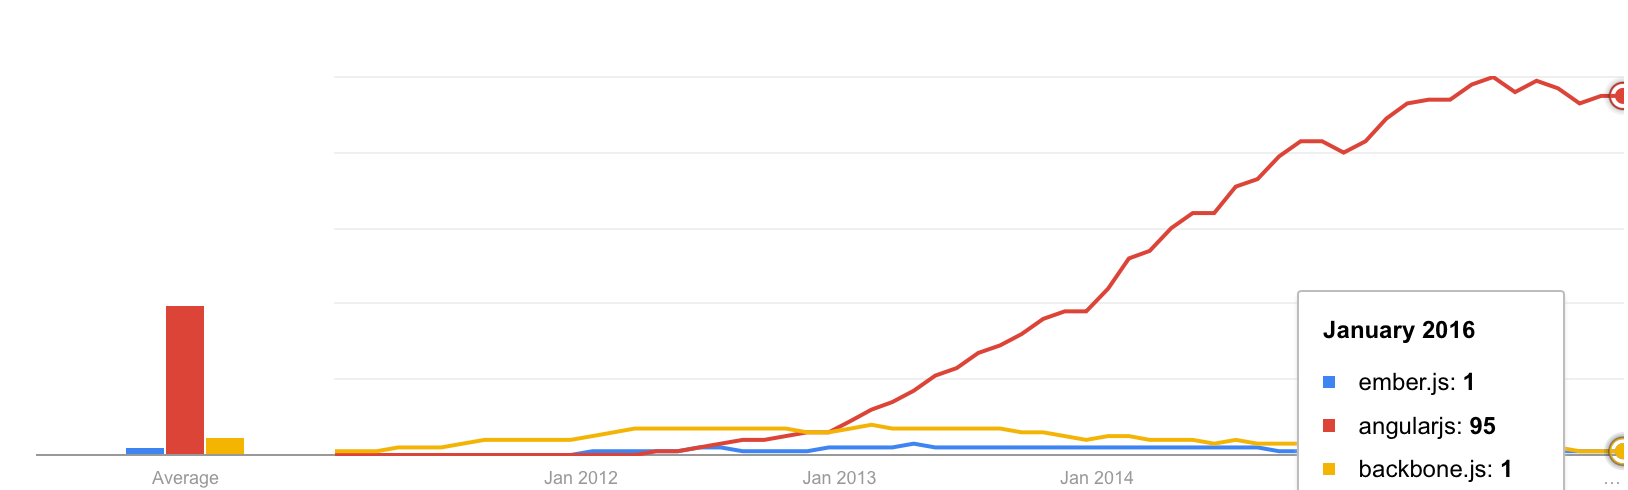
\includegraphics[width=150mm]{Quellen/Google_Trends_angular_und_co.png}
	\caption{Google Trends Angular, Backbone, Ember 01.2011-01.2016}
	\label{img:google_trends_angular}
\end{figure}
Da dies die meistgenutzten Webseiten der Communities im Kontext der Webentwicklung sind ist eine Zuhilfenahme dieser zumindest ein interessanter Indikator. Betrachtet man die Google-Suchanfragen innerhalb der vergangenen 5 Jahre in Abbildung \ref{img:google_trends_angular}\footcite{analytics_angular} dann fällt auch hier die Skala ganz zu Gunsten von AngularJS. Auch was das Wachstum der Nutzer angeht liegt AngularJS weit vor seinen Konkurrenten. (vgl. \cite{funnyant_mvc_comparison})
\\Doch die Community ist bei weitem nicht der einzige Faktor nach dem ein Framework ausgewählt werden sollte. Deshalb werden im Folgenden AngularJS, Backbone.js und Ember.js in größerem Detail vorgestellt um eine differenziertere Entscheidung treffen zu können.
   \subsubsection{AngularJS}
AngularJS kommt grundsätzlich ohne zusätzliches Framework-Vorraussetzungen aus. Das meint dass zur Einbindung von AngularJS in ein Webprojekt kein anderes Framework benötigt wird. Dieser Umstand führt zu einer Gesamtgröße der runterzuladenden Dateien von 33kb (Stand 2013). Diese Größe sollte in die Bewertung einfließen, da sie Teil des Code-Inhalts ist, der von jedem Nutzer der Webseite bei initialem Aufruf temporär heruntergeladen wird. Sie trägt also zur Gesamt-Performanz bei. Angular-Programmierern ist es zudem ohne Probleme möglich, auch andere Frameworks zusätzlich zu nutzen. Das heißt das die Nutzung von AngularJS das Projekt nur sehr gering gegenüber anderen Javascript-Frameworks vorbelastet. Verständlicherweise untertützt Angular nicht, dass im Projekt andere MVC-Frameworks genutzt werden aber die Einbindung der populärsten Frameworks wie zum Beispiel Jquery ist nicht nur ohne Probleme ermöglicht sondern von Angular sogar explizit unterstützt. So hat das Angular-Team zur Nutzung von Jquery sogar eine abgespeckte Version dessen schon in das Framework integriert. 
   \subsubsection{Backbone}
  \subsection{Resultat}
 \section{Frontend-Layout Framework}
  \subsection{Anforderungen}
  \subsection{Analyse}
   \subsubsection{Bootstrap}
   \subsubsection{Angular Material}
  \subsection{Resultat}
 \section{Grafische Darstellung von Statistiken}
  \subsection{Anforderungen}
  \subsection{Analyse}
   \subsubsection{D3.JS}
   \subsubsection{Chart.js}
   \subsubsection{Morris.JS}
  \subsection{Resultat}
\chapter{Umsetzung}
 \section{Infrastruktur}
  \subsection{Routing}
  \subsection{Services}
  \subsection{Optimierungen}
 \section{Visualisierung}
  \subsection{Aufbereitung der Daten}
  \subsection{I/O}
 \section{Entwicklungspotential}
\chapter{Zusammenfassung und Ausblick}



% ---------------------------- Literaturverzeichnis ----------------------------------------------
\printbibliography

% ------------------------------- Anhang ---------------------------------------------------------

\begin{appendix}
\clearpage
\pagenumbering{Roman}						% römische Seitenzahlen für Anhang
\end{appendix}


\end{document}
